\chapter{De-Entanglement by Priors - Case study with Acoustic Unit Discovery}

\section{Problem Introduction}
A major bottleneck in the progress of many data-intensive language processing tasks such as speech recognition and synthesis is scalability to new languages and domains. 
Building such technologies for unwritten or under-resourced languages is often not feasible due to lack of annotated data or other expensive resources. 
A fundamental resource required to build such a stack is a phonetic lexicon - something that translates acoustic input to textual representation. Having such a lexicon, even if noisy, can help bootstrap speech recognition models, synthesis, and other technologies. Typical approaches may involve a pivot language or bootstrapping or adapting from a closely related high-resource language.
But, this can be a deceptively non-trivial task due to linguistic differences which can pose inherent difficulties. 
For instance, it may be unreasonable to analyze a Sino-Tibetan language using English as a source. Moreover, using an additional language might make the model learn unintended surface level associations or biases between the participating languages that prevent them from generalizing across languages. Associations between these languages over a set of units that may better generalize to other languages. Therefore, in this paper we are interested in discovering the appropriate acoustic phonetic units. 

\begin{figure}[t]
\centering
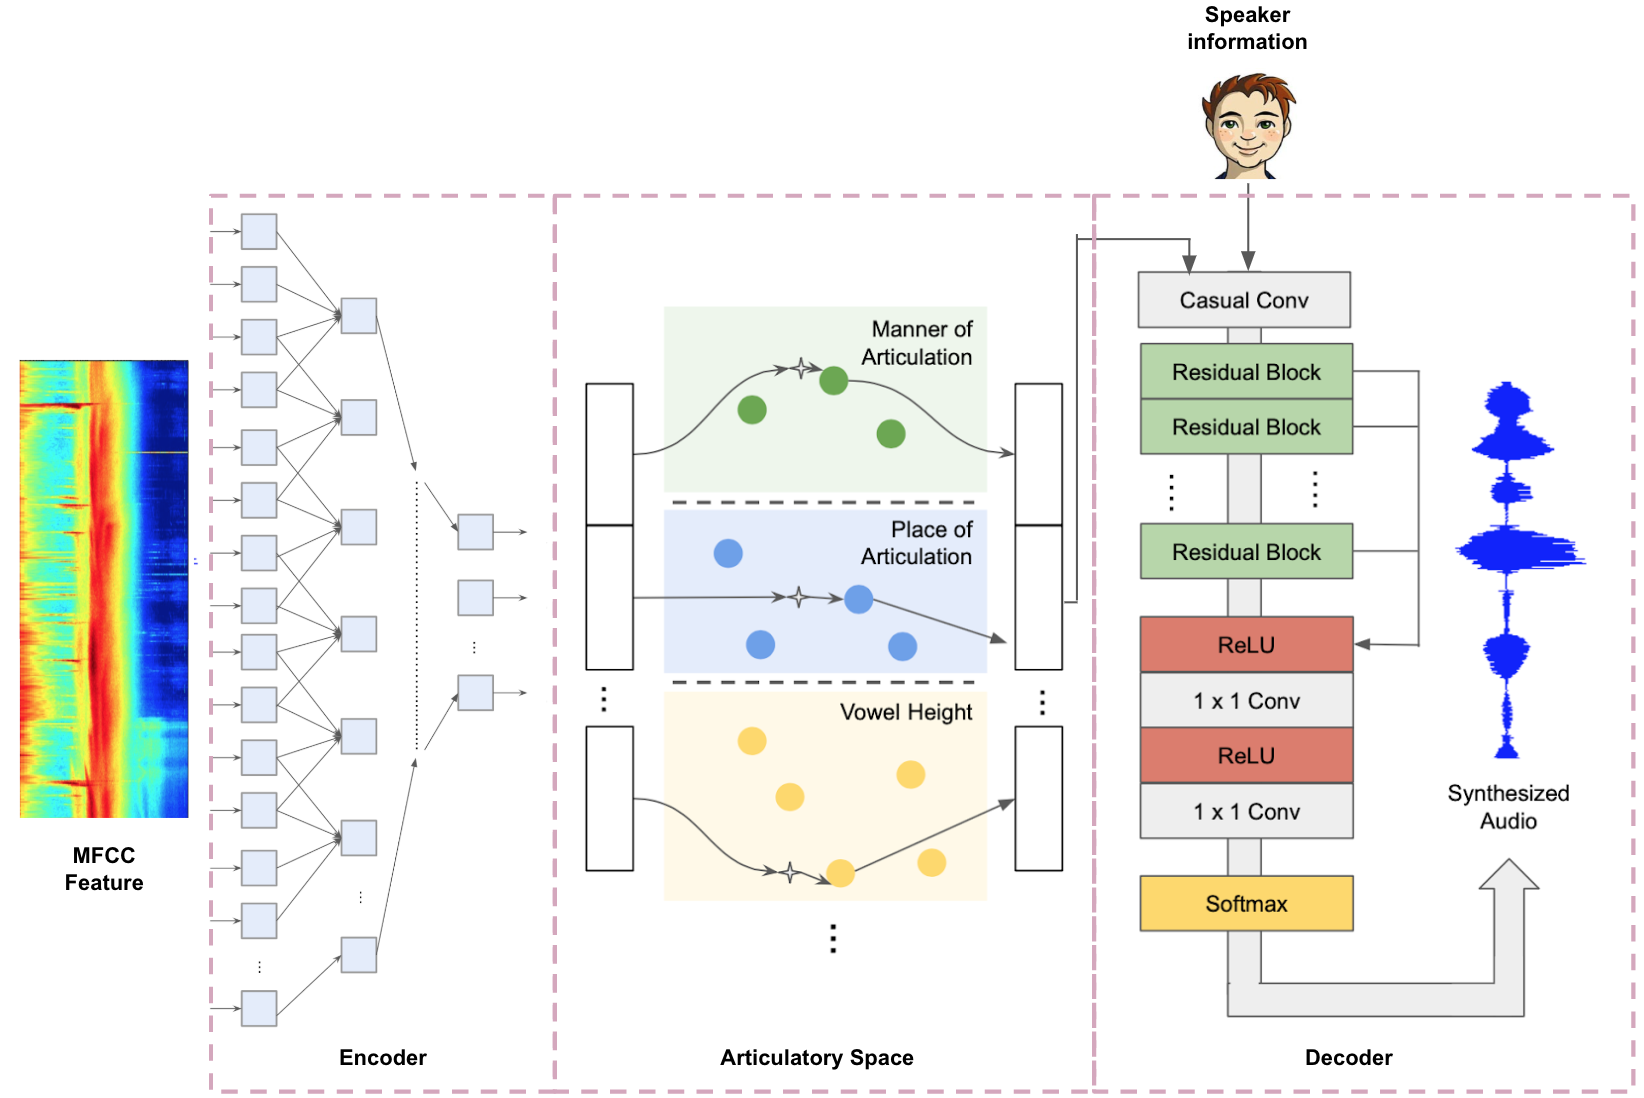
\includegraphics[width=80mm,scale=0.5]{images/vaconda_architecture_zerospeech2019.png}
\caption{Illustration of our procedure for automatically discovering acoustic units from a speech utterance. We pass the speech utterance through a downsampling encoder. The encoded representation is hashed to a latent code based on a discrete articulatory prior bank. The code is passed to the decoder, a WaveNet using speaker embeddings as global conditioning that regenerates audio. } 
\label{frame_replacement_overview}
\end{figure}  


In ZeroSpeech Challenge\citep{zerospeech2019} resynthesis is considered a good proxy task to evaluate the performance of systems when training using unsupervised approaches. To accomplish this we use neural generative models. %Resynthesis might be a good proxy. 
Deep Neural Generative models have seen a tremendous amount of progress in the recent past. These models aim to model the joint probability of the data distribution and the conditioning information as a product of conditional distributions. Typical implementations of such models follow an autoregressive framework, although other formulations have been suggested as well. Such models have been shown very effective in addressing one of the major challenges with conventional vocoding techniques - fidelity. 
Neural generative models has been shown to generate speech that rivals natural speech when conditioned on predicted mel spectrum \citep{shen2017natural}. Speech has a lot of natural variations in terms of content, speaker, channel information, speaking style, prosodic variations, etc. Accordingly, we are interested in models which have flexibility to  marginalize such variations but preserve the phonetic content and distinguish meaningful differences between phonetic units.To accomplish this, we employ sequence to sequence models with latent random variables (referred to as latent stochastic models hereafter). These models provide a mechanism to jointly train both the latent representations as well as the downstream inference network. They are expected to both discover and disentangle causal factors of variation present in the distribution of original data, so as to generalize at inference time. While training latent stochastic models, optimizing the exact log likelihood can be intractable. To address this, a recognition network is employed to approximate the posterior probability using reparameterization \citep{vae}. When deployed in encoder-decoder models, this approach is often subject to an optimization challenge referred to as KL-collapse \citep{bowman_continuous}, wherein the generator (usually an RNN) marginalizes the learnt latent representation. Typical approaches to dealing this issue involve annealing the KL divergence loss~\citep{bowman_continuous,zhou2017multi}, weakening the generator \citep{zhao2017learning} and ensuring the recall using bag of words loss.  In our work, we present an approach to deal with the KL-collapse problem by vector quantization in the latent space.  Building on \citep{vq-vae, chorowski2019unsupervised}, we add additional constraints in the prior space forcing the latent representations to follow articulatory dimensions: The encoded representation is hashed to a latent code based on a articulatory prior bank designed using a discrete codebook. Our decoder is a conditional WaveNet using speaker embedding as global embedding trained to regenerate input audio using the  code sequence as local information. 


\section{Background - Acoustic Unit Discovery}

Let us consider a speech corpus X which consists of speakers $\{ s_1, s_2...,s_n \}$. The goal of acoustic unit discovery is to come up with a set of units \textbf{U} that represent a speech utterance \textit{x} $\subset$ X allowing robust resynthesis. %comprehensively. 
The elements of such a set also might conform to desirable characteristics  such as being injective, consistent and compact, i.e. that different inputs should have discriminant acoustic units, but expected variance such as speaker or dialect should produce the same acoustic units. %, and the set of units should be 
% We aim to discover a minimal set of units to fit these goals.
%must be well corresponding to the acoustic vectors(predictable)


There have been numerous attempts to discover such acoustic units in an unsupervised fashion. In \citep{subword_diarization}, authors presented an approach to modify the speaker diarization system to detect speaker-dependent acoustic units. \citep{unsupervised_AMtraining_ArenJansen} proposed a GMM-based approach to discover speaker-independent subword units. However, their system requires a separate Spoken Term Detector. Recently, due to the surge of deep generative model, using unsupervised method such as auto-encoder and variational auto-encoder (VAE). \citep{badino_autoencoder} designed a stacked AutoEncoder using backpropagation and then cluster the representations at the bottleneck layer. To avoid quick transitions leading to repeated units, they employed a smoothing function based on transition probabilities of the individual states. \citep{hmm-vae_bhiksha} extended the structured VAE to incorporate the Hidden Markov Models as latent model. \citep{vq-vae, chorowski2019unsupervised} proposed VQ-VAE and argue that by vector quantization the ``“posterior collapse" problem could be circumvented.


\section{\textit{VACONDA}}
\label{proposed_approach}


\subsection{Analysis of optimization and de-entanglement}
\label{analysis}

WaveNet \citep{van2016WaveNet} is an autoregressive neural model with a stack of 1D convolutional layers that is capable of directly generating audio signal. It has been shown to produce generated speech that rivals natural speech when conditioned on predicted mel spectrum \citep{shen2017natural}. The input to WaveNet is subjected to corresponding gated activations while passing through each dilated convolutional layer and is classified by the final softmax layer into a $\mu$ law encoding.  The concrete form of the residual gated activation function is given by following equation:


\begin{equation} \label{WaveNet_Eqn}
\begin{split}
  r_d(x) = tanh(W_{f} * x) \odot \sigma (W_{g} * x)  \\ 
\end{split}
\end{equation}

\noindent where $x$ and $r_d(x)$ are the input and output with dilation $d$, respectively. The symbol $*$ is a convolution operator with dilation $d$ and the symbol $\odot$ is an element-wise product operator. $W$ represents a convolution weight. The subscripts $f$ and $g$ represent a filter and a gate, respectively. The joint probability of a waveform \textbf{X} can be written as:


\begin{equation} \label{WaveNet_gen_Eqn}
\begin{split}
  P(X | \theta)  = \prod_{t=1}^{T} P(x_t | x_1, x_2 .. x_{t-1}, \theta)  \\
\end{split}
\end{equation} 

\noindent given model parameters $\theta$. During implementation of WaveNet, the autoregressive process is realized by a stack of dilated convolutions. The final output $y_t$ at time step $t$ can be expressed mathematically as:

\begin{equation} 
\begin{split}
  \hat{y_t} \sim \sum_{d=0}^{D} h_d * r_d(x) \\
\end{split}
\label{WaveNet_Eqn}
\end{equation} 

\noindent where $x$, $y$ represent input and output vectors; $D$ is the number of different dilation used and $d$ is the dilation factor; $h_d$ is the convolution weights. This stack of convolutions is repeated multiple times in the original WaveNet. Optimization in WaveNet is performed based on the error between predicted sample and the ground truth sample conditioned on previous samples in the receptive field alongside the local conditioning. Expressing the loss function being optimized mathematically the error at sample $t$ is:


\begin{equation} \label{discrete_Eqn}
\begin{split}
  l_t = Div(\hat{y_t} || y_t)
\end{split}
\end{equation} 

Here, we define the divergence similar to the \citep{salimans2017pixelcnn++}, To optimize this loss, the contribution from the individual convolution layers towards this global error function must be nullified. Now let us consider the expression for intermediate output for a single filter in Eqn~\ref{WaveNet_Eqn}:

\begin{equation}
\begin{split}
  x_{out}(t) = \sum_{\tau=0}^{t} h(\tau)x(t-\tau)
\end{split}
\end{equation} 

\noindent where $\tau$ is the receptive field covered by the model and $h(\tau)$ represents the discrete state representation at time $t$. Without loss of generality and dropping the term $\tau$ for brevity, the spectral representation generated by the model can be expressed as:

\begin{equation} \label{transfer_function_representation}
  Y(z)  = H(z) X(z) 
\end{equation} 


Considering the discrete nature of input from Eqn \ref{discrete_Eqn}, an interpretation of Eqn \ref{transfer_function_representation} is that the neural autoregressive model acts as the transfer function and is discretized by convolving with the samples from original signal. It has to be noted that this is similar to the formulation of source filter model of speech, specifically the periodic components aka voiced sounds. Voiced sounds typically represented as impulse train are convolved with the transfer function to generate spectral envelope. As a corollary, from Eqn \ref{discrete_Eqn} and \ref{transfer_function_representation}, we posit that the optimization in WaveNet model is performed by minimizing the divergence between true and approximate spectral envelope. Note that latent stochastic models such as VAEs are aimed to minimize the divergence between true and approximate posterior distributions of input data. The advantage with such models is the presence of stochastic random variables that capture the causal factors of variation in input based on some prior information about the distributional characteristics of data. Techniques aimed at this \citep{beta_vae} have shown that it is possible to effectively disentangle the factors of variation using stochastic variables. Hence, we postulate that it should be possible to augment WaveNet decoder with a suitable encoder and an appropriate prior distribution to disentangle the acoustic phonetic units from a given utterance. 


However, this is a deceptively non-trivial task. If the prior is too simplistic, such as unit normal distribution, the model is trivially incentivized to force the posterior distribution to closely follow the Gaussian prior distribution \citep{lossy_vae}, particularly early in training. This results in the decoder marginalizing out the latent variable completely, manifesting in poor reconstruction ability. On the other hand, making the prior distribution arbitrarily complex also leads to unreasonable constraints on the decoder. For instance, in scenarios that have categorical distributions as their output (tasks such as language modeling, machine translation, and image captioning among others) it is unintuitive to assume that the true prior that generates latent distribution is a Gaussian when the likelihood is based on discrete sequential data. We make an observation that dealing with speech presents a characteristic advantage - speech has both continuous as well as discrete priors. The generative process of speech assumes a Gaussian prior distribution which is continuous in nature. However, the language which is also present in the utterance can be approximated to be sampled from a discrete prior distribution. Exact manifestation of this in the linguistics can be at different levels: phonemes, words, syllables, subword units, etc. From the analysis presented in the previous section, we hypothesize that if we use background knowledge about the data distribution while designing the priors, we can help the encoder effectively disentangle the latent causal factors of variation in the data. In other words, this presents us with an opportunity to control what gets disentangled in the latent space by appropriately choosing a prior distribution. Therefore, we engineer our prior space to account for the phonetic information in the utterance by representing the prior as a discrete latent variable bank, similar to the filterbanks used for feature extraction from speech. Each discrete latent variable has a different set of states reflecting one of the articulatory dimensions. The specific design of our latent space is highlighted in Table \ref{articulatory features}.


\renewcommand{\arraystretch}{1.0}
\begin{table}[t]
\caption{Articulatory Features\label{tab:arti}}
\centering
\begin{tabular}{l | c | c}\toprule[\heavyrulewidth] \textbf{Feature name} & \textbf{Value} & \textbf{Details} \\
\toprule[\heavyrulewidth]
vc & + - 0 & vowel or consonant \\
vlng & s l d a 0 & vowel length\\
vheight & 1 2 3 0 - & vowel height \\
vfront & 1 2 3 0 - & vowel frontness\\
vrnd & + - 0 & lip rounding\\
ctype & s f a n l r 0 & consonant type \\
cplace & l a p b d v g 0 & place of articulation \\
cvox & + - 0 & consonant voicing\\
asp & + - 0 & consonant voicing\\
nuk & + - 0 & consonant voicing\\
\bottomrule[\heavyrulewidth]
\end{tabular}
\label{articulatory features}
\end{table}



\section{Experiments}
\label{expts}


\subsection{ZeroSpeech 2019 dataset}
% The goal of ZeroSpeech dataset is to learn the Phonetic representation of the audio without any supervision, discover the symbolic representation of the audio, and resynthesize the audio using these unit. The evaluation metric look at both the quality of sub-unit and the resynthesized audio.

ZeroSpeech Challenge 2019: TTS without T is to propose to build a speech synthesizer without any text or phonetic labels~\citep{sakti2008development1, sakti2008development2, zerospeech2019}. The systems are required to extract the symbolic representation of the raw audio, and then re-synthesize the audio using these discovered units. There are three datasets in total: (1) \textit{Unit Discovery Dataset} provides audio from a variety of speakers and is used to unsupervised acoustic modeling, (2)  \textit{Voice Dataset} provides audio from the targeted speaker and is used for synthesizer modeling and (3)  \textit{Parallel Dataset} is intended for finetuning both the sub-systems. We have not utilized the parallel dataset for our observations in this study. The development language is English and the test language is Standard Indonesian. The system is constrained to not use any pre-existing resource or models. To ensure that the model generalizes out of the box, the hyperparameter will be fine-tuned only on the development dataset, and the model will be trained in test language under the same parameters. 

\iffalse
\begin{enumerate}
    \item \textit{Unit Discovery Dataset} provides audio from a variety of speakers and is used to unsupervised acoustic modeling
    \item \textit{Voice Dataset} provides audio from the targeted speaker and is used for synthesizer modeling
    \item \textbit{Parallel Dataset} is used for finetuning the both sub-systems
\end{enumerate}

The development language is English and the test language is Standard Indonesian. The system is refrained from using any pre-existing resource or models. To ensure that the model generalizes out of the box, the hyper-parameter will be fine-tuned only on the development dataset, and the model will be trained in test language under the same parameters. 
\fi

% \subsubsection{CSTR VCTK Corpus}

% CSTR VCTK is an English speech dataset, which contains 109 native speakers with various accents. Each speaker is required to record 400 sentences from newspaper, plus Rainbow Passage and an elicitation paragraph intended to identify the speaker's accent.

%\subsection{Implementation Details}

% CSTR VCTK Corpus includes speech data uttered by 109 native speakers of English with various accents. Each speaker reads out about 400 sentences, most of which were selected from a newspaper plus the Rainbow Passage and an elicitation paragraph intended to identify the speaker's accent
% 
% newspaper sentences,

\iffalse
Our voice building process employs the phone sharing approach as outlined in \citep{rallabandi_mixedlingual_IS2017} - where the combined phoneset is formed by the union of phones from both the languages - to build acoustic models. In this section, we present our approaches to generate the required bilingual acoustic data using just monolingual recordings. Specifically, in each of the subsections, we introduce the approaches we follow to artificially generate spectral content in English. We then follow the outlined procedure to build a bilingual voice using the native (L1) recordings and `pseudo English' (L2) recordings. 

In this section, present our approaches for ZeroSpeech 2019. Specifically, our aim is to build robust models capable of accomplishing (1) Discovering acoustic units given a speech utterance. and (2) Generating novel utterances conditioned on the discovered acoustic units. For this, we have built two systems: (1) System A which is a pipeline based approach and (2) System B which is an end-to-end approach. 
\fi 

\section{Baseline System}

We have a three-stage pipeline: (1) \textit{Unit Discovery}: We hypothesize acoustic units given a speech utterance using latent Stochastic Models; (2) \textit{Unit Alignment}: We fine-tune the alignment between the utterance and the proposed acoustic units ; (3) \textit{Unit Synthesis}: We build a speech synthesizer using the acoustic units and the target voice.


%In this section, we will elaborate on each of the three stages.

%\subsubsection{Acoustic Unit Discovery}
%\subsubsection{Acoustic Unit Alignment}

As proposed in \citep{sitaram2013bootstrapping}, we take the initially discovered transcription of the acoustic units for our speech corpus and train an ASR model on it. Then we re-encode the corpus using the ASR model, and train a TTS system on it. Here we using Bi-LSTM with CTC loss as our ASR model, and tacotron \citep{tacotron_transferlearning2multispeaker} as TTS system. 

% At each iteration, an acoustic model is trained from the parallel speech-transcription data. This acoustic model is then used to re-decode the speech data, and so on for 10 iterations. At the end of each iteration, we have produced a rebuilt acoustic model and a re-decoded transcript. These two are used to build a synthetic CLUSTERGEN \citep{black2006clustergen} voice (given the noise in the generated data, statistical parametric synthesis is appropriate) using Festvox for the purpose of evaluation on a held out test set on the basis of MCD scores. The best-aligned transcription is taken as the one producing the synthetic voice with the lowest distortion score.

%\subsubsection{Acoustic Unit Synthesis}





\begin{figure}[t]
  \centering 
  \subfigure[Original speech]{ 
    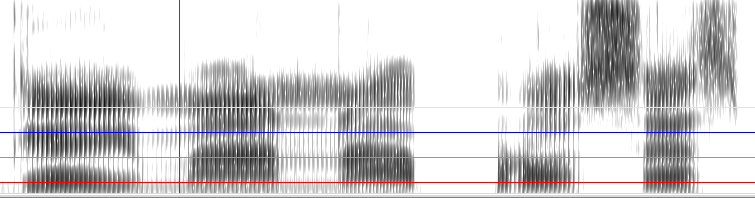
\includegraphics[width=0.95\linewidth]{images/target4.png}}
\subfigure[Generated speech]{
    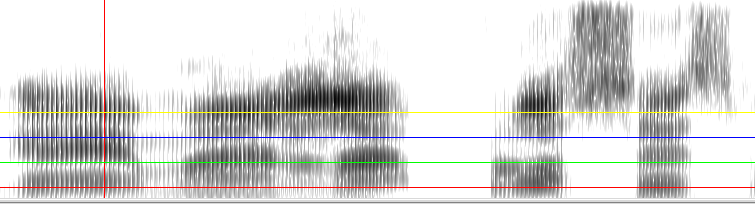
\includegraphics[width=0.95\linewidth]{images/generated4.png}}
\subfigure[Converted speech]{
    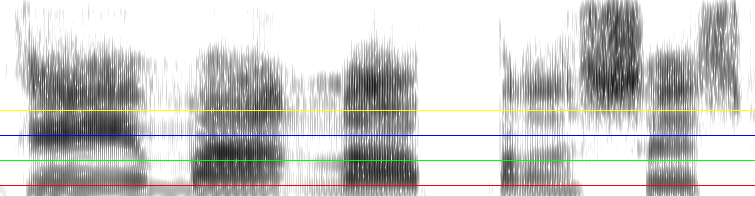
\includegraphics[width=0.95\linewidth]{images/transferred4.png}}
  \caption{Spectrograms of original, generated, and converted speech. The source speaker is female while the target speaker is male.\label{fig:waveform}}
\end{figure}


\subsection{VACONDA}

The architecture of our model is built on top of VQ-VAE. It consists of three modules: an encoder, quantizer and a decoder. As our encoder, we use a dilated convolution stack of layers which downsamples the input audio by 64. The speech signal was power normalized and squashed to the range (-1,1) before feeding to the downsampling encoder. To make the training faster, we have used chunks of 2000 time steps. This means we get 31 timesteps at the output of the encoder. The quantizer acts as a bottleneck and performs vector quantization to generate the appropriate code from a parameterized codebook. We define the latent space $e \in \mathbmm{R}^{k\times d}$ to contain $k$ $d$-dim continuous vector. Quantization is implemented using minimum distance in the embedding space. The number of classes was chosen to be 64, approximating 64 universal phonemes. We use a linear mapping to first project the 128 dimensional vector to 160 dimensions. We then perform comparisons with respect to individual articulatory dimensions each of which is 16 in size.  Assuming $z_e(x)$ denotes the encoder output in the latent space, then the input of decoder $z_d(x)$ will be obtained by $\argmin_{j}d(e_j, z_e(x))$, where $d$ is a similarity function of two vectors. In this paper, we consider Euclidean distance as the similarity metric.  Our decoder is an iterated dilated convolution-based WaveNet that uses a 256-level quantized raw signal as the input and the output from vector quantization module as the conditioning. Although using a Mixture of Logistics loss function might yield a better output, we have only used a 256 class softmax in this study. The decoder takes the output from the quantizer along with the speaker label as global conditioning and aims to reconstruct the input in an autoregressive fashion. Following IDCNNs, we have shared the parameters of all the stacks.



% In this subsection we describe our end-to-end approach for the task. We extend the framework proposed in \citep{vq-vae} to accomplish subword unit discovery. Although a structure such as HMM \citep{hmm-vae_bhiksha} might be intuitively better at capturing the transitions, we have limited ourselves to a vector quantization based approach as we observed it to be better at handling the posterior collapse problem in VAEs. We have used 3 stacks of 10 layers each in the decoder and residual blocks with similar dilation factors in each of the stacks shared their parameters \citep{strubell2017fast}.

% Our voice building process employs the VQ-VAE approach as outlined in \citep{rallabandi_mixedlingual_IS2017}, where the raw audio is first fed to a downsampling encoder which reduces the time resolution by 64. This encoded representation is then hashed into a latent representation that is forced to follow articulatory constraints. Specifically, we employ a set of discrete embeddings of cardinality 5, where each is a multi-dimensional array in itself associated with a continuous vector. The output from this hash function is fed to the decoder, which is a conditional WaveNet implemented using iterated dilated convolutions. In this section, we first present our analysis of the optimization that happens in our models. We then present a case for controlling the disentanglement that happens in such models to accomplish voice conversion. This is followed by an explanation of each component in our model in detail.

% Aside from the architecture discussed in Section~\ref{proposed_approach}, we argue that adding meaningful inductive bias can help the model learn better. We first normalize the vector representation to ensure the same scale in the latent space. Compared to VQ-VAE, we incorporate the articulatory features information in Table~\ref{tab:arti}. The above articulatory features apply to all human languages. To incorporate them, we first transpose the embedding from 128-dimension to 160-dimension by a linear layer. Then, we equally divide the latent embedding into 10 parts, and perform the vector quantization separately. Finally we concatenate all vectors, and feed into the linear layer to map it back to 128-dimension. In each class, the number of latent embedding is the number of possible values.


\subsection{Analysis}

In this section, we will discuss different design choices in the architecture, including input features and latent space constraints. 

% \subsubsection{Input Feature}

% We first compare the performance gap between different features as our model's input. The feature used along with its performance is shown in Table~\ref{tab:input}.

\subsubsection{Acoustic Unit Discovery}

Here we analyze the AUD performance of three different models in ZeroSpeech dataset as shown in Table~\ref{tab:aud}. We only show the results in English since we don't have ground truth for the Indonesian language.

% Now all is baseline 

\renewcommand{\arraystretch}{1.1}
\begin{table}[!htbp]
\caption{Performance of different systems in ZeroSpeech}
\centering
\begin{tabular}{l c c}\toprule[\heavyrulewidth]
& \multicolumn{2}{c}{English}\\
Model & ABX score & bitrate \\
\toprule[\heavyrulewidth]
Baseline & \textbf{27.46} & 74.5\\
Three-stage Model & 34.86 & 68.54 \\
VACONDA & 38 & \textbf{58.19} \\

\bottomrule[\heavyrulewidth]
\end{tabular}
\label{tab:aud}
\end{table}

As in Table~\ref{tab:aud}, the VACONDA achieves the best bit rate among three models. With such small number of unit, we could resynthesize and even convert the speech in a very high quality.

\subsubsection{Speech Resynthesis and Conversion}

The proposed model supports synthesizing the same speech in both the same speaker and a different speaker. Here we show a sample in the test dataset of Indonesian language in Figure~\ref{fig:waveform}. When we feed the decoder with the same speaker identification, the decoder will generate the original audio. Otherwise, it will perform speech convertion. The three audio shares similar structure.  However, the converted audio has denser waveform, suggesting it's a different speaker. For the sampled audio, please visit the \href{http://tts.speech.cs.cmu.edu/rsk/campaigns/interspeech2019/submissions/acoustic_unit_discovery/}{our website}.



%The results are shown in Table~\ref{tab:constraints}. We use 

% \renewcommand{\arraystretch}{1.1}
% \begin{table}[htbp]
% \caption{System performance with latent space constraints}
% \centering
% \begin{tabular}{l | c}\toprule[\heavyrulewidth] \textbf{Model} & \textbf{ABX score}\\
% \toprule[\heavyrulewidth]
% Baseline model & 12\\
% \bottomrule[\heavyrulewidth]
% \end{tabular}
% \label{tab:constraints}
% \end{table}

\label{analysis}


\subsection{Conclusion}

In this case study, we present an approach to automatically discover acoustic-phonetic units from a speech utterance in an unsupervised fashion. We first present an analysis to show that incorporating latent random variables into neural generative models using suitable priors allows us to control what gets encoded into the latent space. Based on this, we employ articulatory features as a discrete prior bank in the latent space and obtain acoustic units that are speaker and language independent.  To validate effectiveness of the discovered units, we perform discriminability tests as part of ZeroSpeech Challenge 2019. 
